% English version of paper/ja_v2/01_序論.md (2026-11-17). Numbers: see the source comments in the Japanese file.
\section{Introduction}\label{sec:intro}

Corpora for multimodal emotion recognition (MER) differ in how emotions were elicited, recorded and labelled. IEMOCAP records improvised and scripted dyadic sessions of actors in a laboratory \cite{busso2008iemocap}, CMU-MOSEI collects YouTube monologues \cite{zadeh2018mosei}, MELD collects dialogues from a TV series \cite{poria2019meld} and AFEW collects movie clips \cite{dhall2012afew}. Factors that change across corpora and can affect emotion recognition include environmental noise, recording devices, acted versus natural elicitation and speaker demographics \cite{gideon2021addog}, and the corpora also differ in how they were annotated (Table~\ref{tab:corpora}). Emotion classifiers trained on one corpus have been reported to perform worse on other corpora \cite{ryumina2025,gideon2021addog}.

Adapting a classifier to a new corpus requires labels of that corpus, but emotion labels are collected from several raters who watch or listen to each utterance, which is costly to repeat for every new corpus \cite{parthasarathy2020ladder,abdelwahab2018dann}, whereas unlabelled recordings are easy to collect \cite{abdelwahab2018dann}. We consider a new (target) corpus with only a few (K) labels per emotion and treat it as semi-supervised domain adaptation \cite{saito2019mme}, which uses three kinds of data that we call information sources: labelled other corpora (sources), the K target labels and unlabelled target utterances. Methods usable in this problem have been proposed for each information source: aligning source and target representations \cite{ganin2016dann,sun2016coral}, and self-training and entropy minimisation on predictions for unlabelled utterances \cite{lee2013pseudolabel,grandvalet2004,saito2019mme}.

In MER, the other modalities of the same utterance form a fourth information source. Albanie et al.\ \cite{albanie2018} attached the predictions of a facial-expression classifier to unlabelled videos and trained an audio emotion classifier on them, and Zhang et al.\ \cite{zhang2021combining} combined this scheme with semi-supervised learning. We call the four-emotion probabilities that classifiers including other modalities assign to unlabelled utterances \emph{pseudo-labels}, and retraining a classifier towards them without temperature \emph{distillation} \cite{hinton2015distilling,albanie2018} (Sect.~\ref{sec:distill}). When pseudo-labels are built from the predictions of several classifiers (audio, visual and text), one must decide how much weight each classifier's predictions receive; Busso et al.\ \cite{busso2004} reported that audio and visual classifiers recognise different emotions well. However, when the target has only a few labels per emotion, it remains unclear which part of the error each of the four sources corrects, which classifiers distillation improves and when, and how the predictions should be combined into pseudo-labels.

We place linear emotion classifiers on features of frozen pretrained audio, visual and text encoders and split their error into the part where predictions are biased towards some emotions (\emph{answer bias}) and the part that remains after removing that bias (\emph{remaining error}). This setting serves as a diagnostic of what each information source changes in a classifier rather than as a new architecture, and we do not claim that the results hold for fine-tuned encoders (Sect.~\ref{sec:limitations}). We answer three research questions (Fig.~\ref{fig:questions}).
\begin{itemize}
\item \textbf{RQ1(a) (analysis, Sect.~\ref{sec:rq1a}):} Does each of the four information sources (labelled source utterances, K target labels, unlabelled target utterances, pseudo-labels from classifiers including other modalities) correct the answer bias or the remaining error?
\item \textbf{RQ1(b) (analysis, Sect.~\ref{sec:rq1b}):} Does distillation raise the UAR of the audio, visual and text classifiers and of the classifier on their concatenated features (AVT)? Which classifiers gain, and when?
\item \textbf{RQ2 (method, Sect.~\ref{sec:rq2}):} How should the predictions of the audio, visual and text classifiers be combined into pseudo-labels?
\end{itemize}

\begin{figure}[t]
\centering
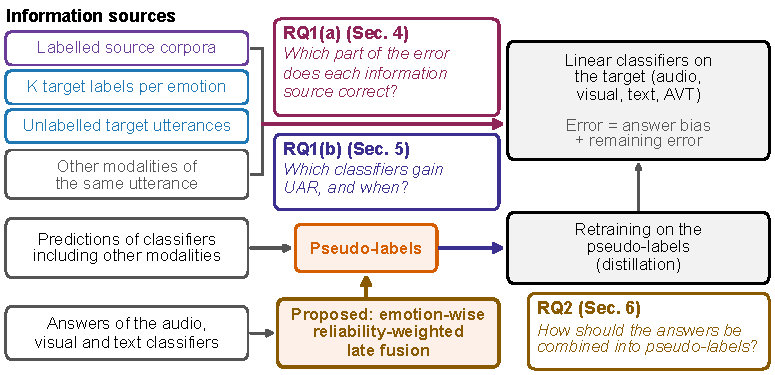
\includegraphics[width=\textwidth]{figures/fig_v2_questions_en.pdf}
\caption{The three research questions, written on the arrows of the processing flow they ask about}\label{fig:questions}
\end{figure}

Our contributions are threefold.
\begin{enumerate}
\item \textbf{We show that, with one source corpus, audio and visual answer bias was almost removed by label-free feature-mean subtraction, whereas with all other corpora as sources, the remaining error was rarely reduced by same-modality unlabelled utterances and was reduced by pseudo-labels from classifiers including other modalities (RQ1(a)).} For audio with K = 5, mean subtraction gained 4.69\pt\ over a classifier trained on one source corpus, close to the 5.26\pt\ of training on the source and the K target labels together. The remaining error was reduced in 38 of 81 conditions by distillation and in 7 of 210 conditions by eight methods using same-modality unlabelled utterances.
\item \textbf{We find that distillation raised the point estimate of audio UAR, and that, in post hoc variants, UAR rose (95\% interval of the difference above zero) only when the pseudo-labels had higher UAR than the classifier before retraining (RQ1(b)).} When each corpus in turn served as the new corpus, the audio classifier had higher UAR than before retraining in all 12 conditions with 5, 10 and 25 labels per emotion (point estimates; 1.4--4.1\pt), and 11 methods that do not use pseudo-labels including other modalities were all lower than distillation in point estimates. Across 360 post hoc pseudo-label variants per K (K = 5, 25; pseudo-labels made only of the retrained classifier's own predictions and duplicates excluded), the rank correlation between the UAR of the pseudo-labels' decisions minus that of the classifier before retraining (the \emph{advantage}) and the UAR difference was 0.80 and 0.83, and none of the variants with a negative advantage (173 and 184) rose.
\item \textbf{Using the finding that the strongest modality differed by corpus and emotion, we propose emotion-wise reliability-weighted late fusion that measures the strength of each classifier on the K target labels and its per-emotion profile on the source corpora (RQ2).} Only three numbers (one strength per classifier) are estimated from the K labels, and hyperparameters are selected on episodes in which each source corpus serves in turn as a provisional target. The UAR of the fused predictions was higher than that of the product of the three probabilities in 11 of 12 conditions (four corpora $\times$ three K; point estimates) and by 2.1--3.5\pt\ on AFEW.
\end{enumerate}

Section~\ref{sec:related} reviews related work and Sect.~\ref{sec:setup} describes the data, features, classifiers and settings shared by the three questions. Sections~\ref{sec:rq1a}--\ref{sec:rq2} each give the setting, results and the answer for one question. Section~\ref{sec:discussion} links the analysis to the method and to prior work, Sect.~\ref{sec:limitations} states limitations and Sect.~\ref{sec:conclusion} concludes.
